% LaTeX file for resume
% This file uses the resume document class (res.cls)

\documentclass[margin]{res}%{moderncv}%{res}
% the margin option causes section titles to appear to the left of body text
\textwidth=5in %  5.2increase textwidth to get smaller right margin
%\usepackage{helvetica} % uses helvetica postscript font (download helvetica.sty)
%\usepackage{newcent}   % uses new century schoolbook postscript font
% use your favourite citation style here
\usepackage{apacite}

% \usepackage[left=2.5cm,right=2.5cm,top=1.5cm,bottom=2.5cm]{geometry}

\usepackage{xcolor}
% as bibentry and hyperref clash in some cases, this is a workaround
% as suggested by the following two links:
%https://tex.stackexchange.com/questions/227933/using-bibentry-to-cite-in-text-reference-with-apacite
% and
%https://tex.stackexchange.com/questions/65348/clash-between-bibentry-and-hyperref-with-bibstyle-elsart-harv/65401#65401
\usepackage{bibentry}
\makeatletter\let\saved@bibitem\@bibitem\makeatother
\usepackage[colorlinks=true, urlcolor={teal}]{hyperref}
\makeatletter\let\@bibitem\saved@bibitem\makeatother




% hanging publications: 1st line starts at beginning of line,
% further lines are placed a bit to the right
\usepackage{hanging}
\newcommand\pub[1]{%
	\smallskip\par\hangpara{1.5em}{1}\bibentry{#1}\smallskip
}



\usepackage{graphicx}




% hanging publications: 1st line starts at beginning of line,
% further lines are placed a bit to the right
\usepackage{hanging}
\newcommand\publication[1]{%
	\smallskip\par\hangpara{1.5em}{1}\bibentry{#1}\smallskip
}



\usepackage{scrextend}

\begin{document}
	% bibliography
	% NB: no .bib extension — BibTeX appends it. With it, BibTeX looks for
	% publications.bib.bib, finds nothing, writes no .bbl, and every
	% \publication{} silently expands to nothing.
	\nobibliography{publications}
	\bibliographystyle{apacite}
%\begin{table}[]
 %   \centering
  %  \begin{tabular}{l c}
 %      Niklas Erdmann  &  \\
  %        &  \\
  %        & \includegraphics[scale=0.08]{pic_cv}\\
  %  \end{tabular}
  %  \label{tab:my_label}
%\end{table}

%\begin{center}
%    Niklas Erdmann\\[12pt]
%\end{center}

%\name{Niklas Erdmann\\[12pt]} % the \\[12pt] adds a blank line after name

%\address{{\bf Address} \\ Saffierstraat 27 \\ 9743 LE, Groningen\\  }
%\address{{\bf Contact} \\ 0612663583 \\ n.erdmann@student.rug.nl  }
 %  \smash{ \includegraphics[width=0.2\textwidth]{pic_cv}}

\begin{minipage}[l]{0.7\textwidth}
\hspace{-3.5cm}
\begin{Large}Niklas Erdmann\end{Large}\vspace{0.4cm}\\
%\hspace*{-3.4cm}\hspace*{-1.7cm}

% \hspace*{-3cm}{\bf Date of Birth:} \hspace*{0.01cm} 12.07.1996\\
% \hspace*{-3cm}{\bf Nationality:} \hspace*{0.02cm} German\\
\vspace{0.2cm}\\
\hspace*{-3.3cm}{\bf Contact:} \hspace*{0.02cm} niklas.erd@gmail.com // niklase@uio.no\\
\hspace*{-1.5cm} \href{https://www.linkedin.com/in/niklas-erdmann-0020b4122/}{linkedin}, \href{https://scholar.google.com/citations?user=zX22NboAAAAJ&hl=en&inst=4058163445224007304}{google scholar}, \href{https://www.mn.uio.no/its/english/people/aca/niklase/}{uio homepage}, \href{https://orcid.org/0009-0004-4533-5741}{orcid}, \href{https://github.com/Coopez}{github}

\end{minipage}
\begin{minipage}{0.3\textwidth}
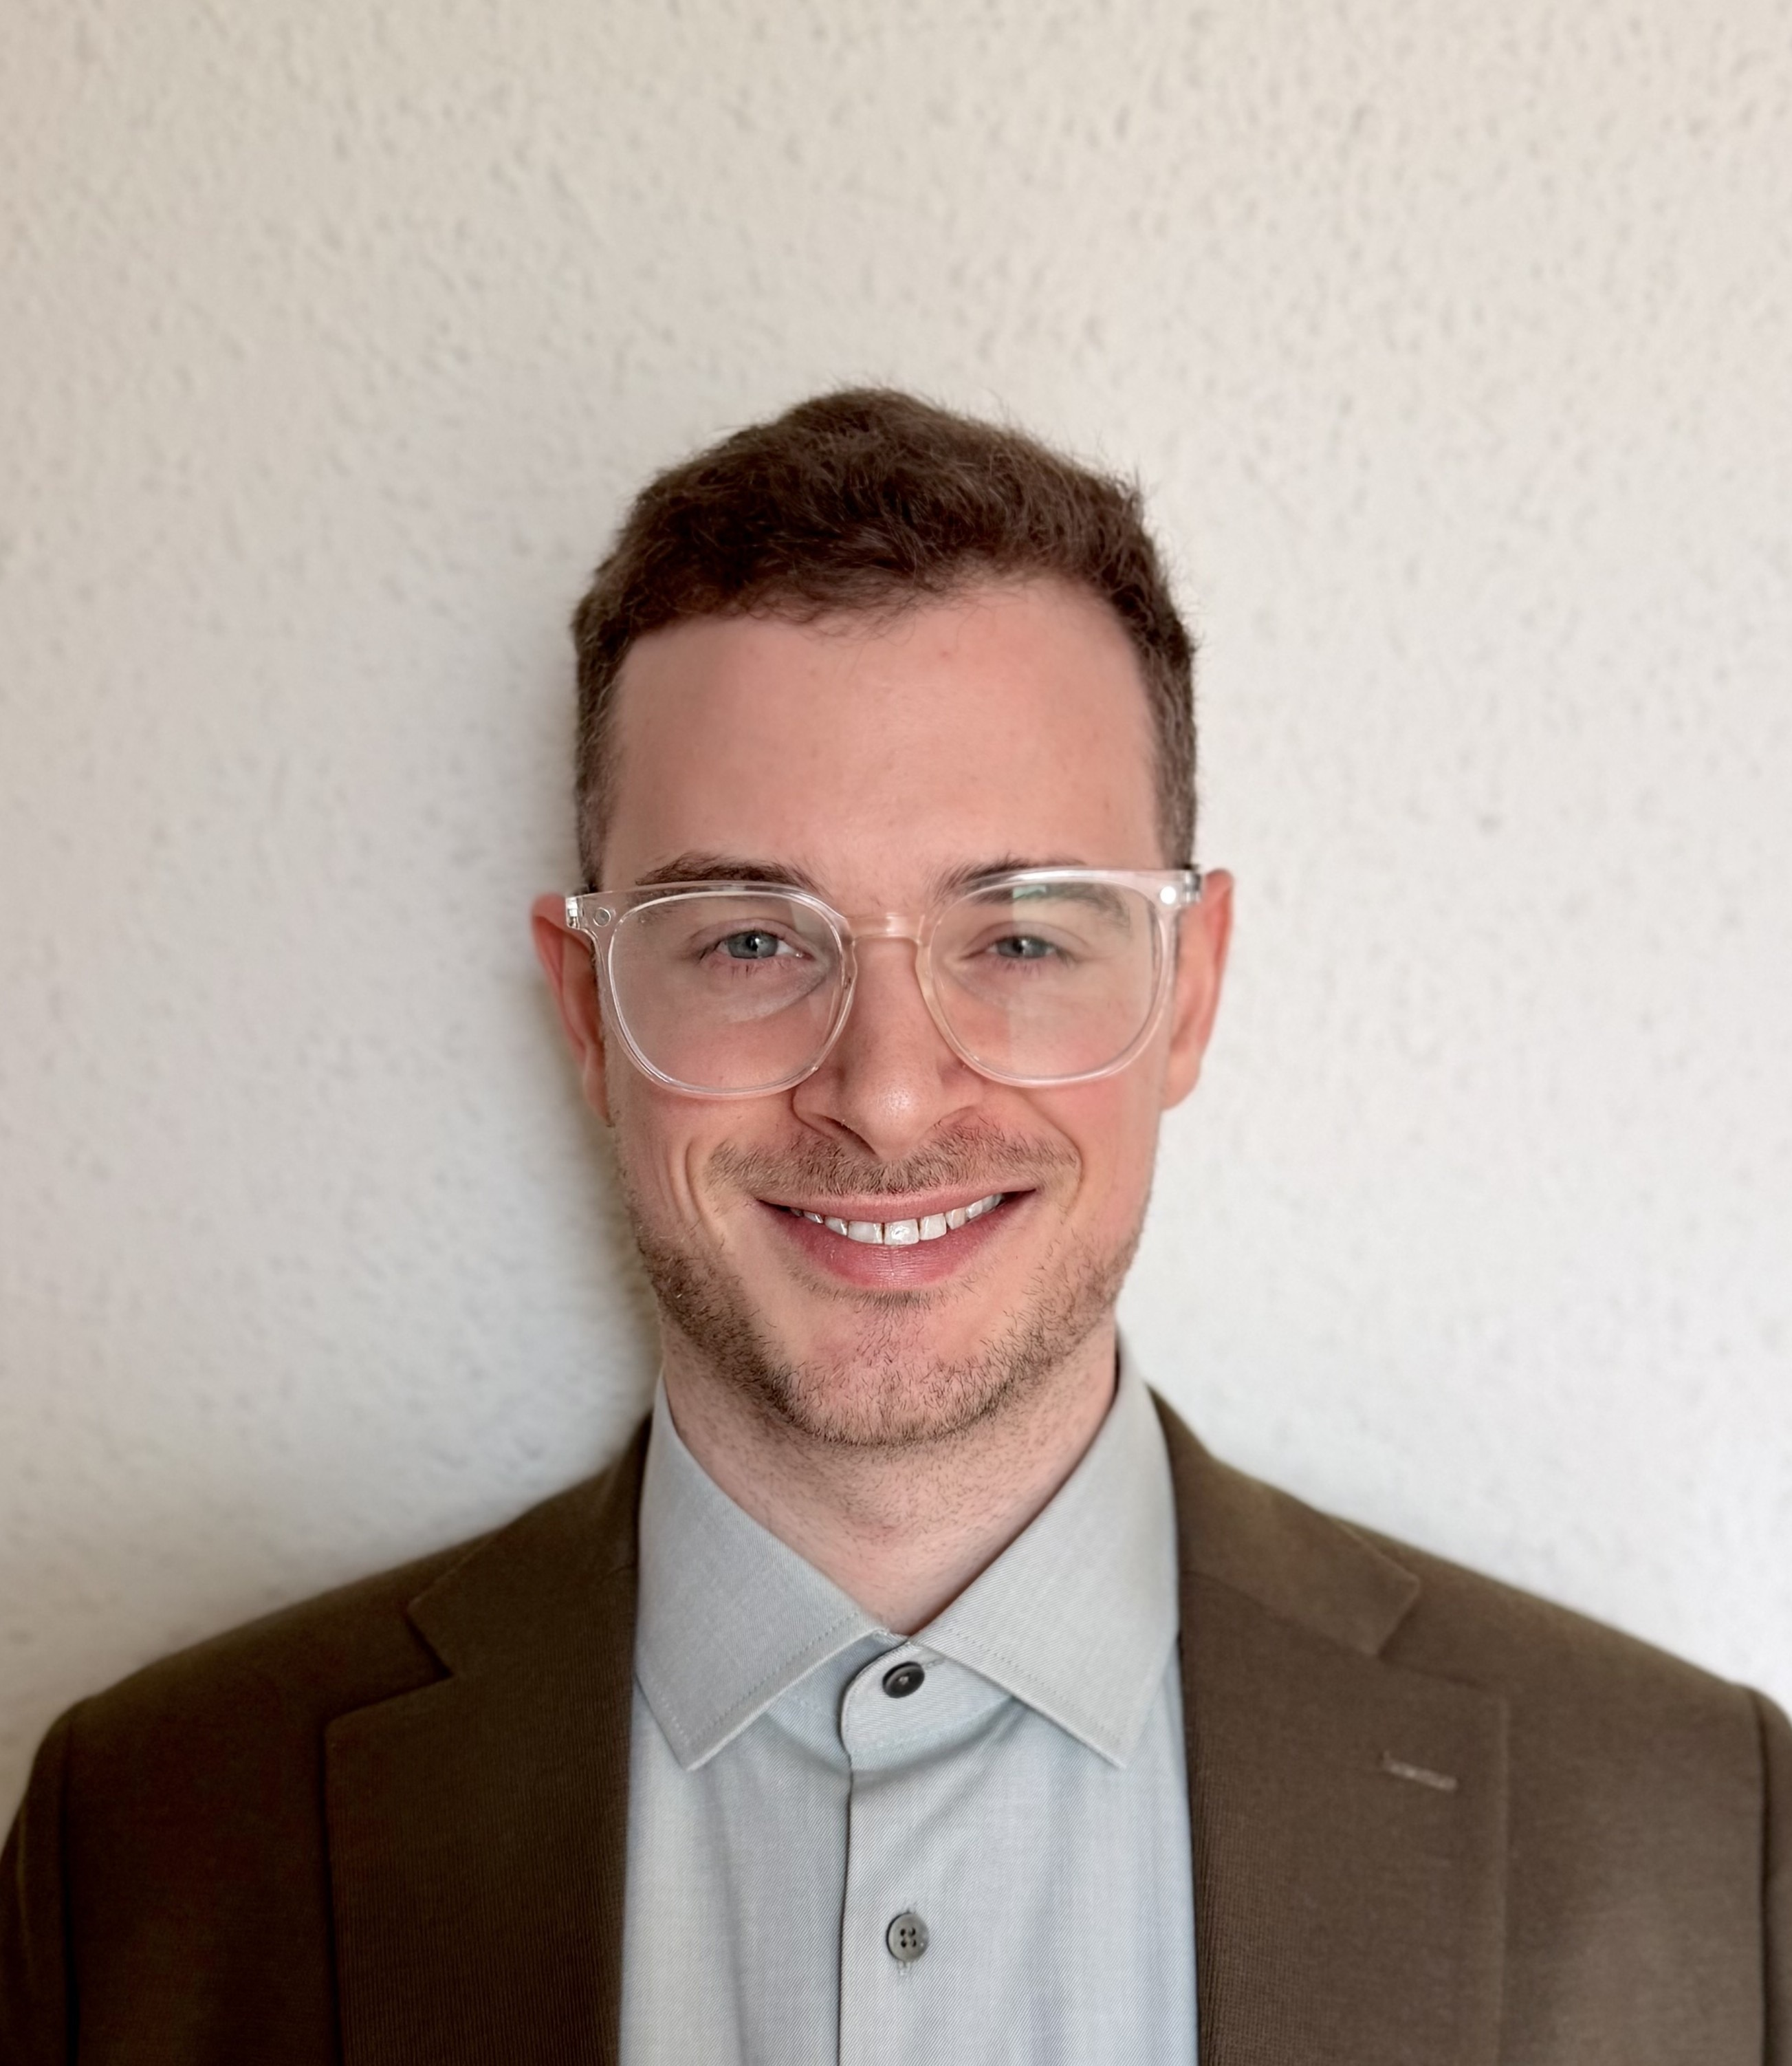
\includegraphics[width=1\textwidth]{formal_frontlight_smaller2.jpeg}
\end{minipage}



\begin{resume}
\section{About Me:}
% What do I want to portrait?
% - strong collaboration experience and interest across diverse fields.
% - diverse background in AI, statistics and social science.
% - broad educational foundation across areas of AI: multi-agent systems, neural networks, and robotics
% - lots of teaching experience
% - strong softskills, writing and experience with the AI training-tuning-testing loop

% specified 50-60 words intro
%Here personal introduction paragraph\\


Personal curiosity, peers, and experiences during my prior education led me to be interested in researching applications of Artificial Intelligence (AI) in our world's problems and to pursue a PhD in Oslo. My experiences, interests, and collaborations enabled me to many cross-disciplinary interactions in which I enjoy contributing with my broad background in AI, Statistics, and Psychology. Continuous passion for research and teaching guides me towards more academic endeavours.

\section{Post-Graduate Education:}
%\href{https://www.rug.nl/masters/artificial-intelligence/?lang=en}{{\bf MSc. Artificial Intelligence}, University of Groningen} \hfill {\bf09.2019 - 07.2022 }   \\

{\bf PhD.}, \href{https://www.mn.uio.no/its/english/}{Dep. of Technology Systems}, University of Oslo  \hfill {\bf03.2023 - 03.2027 }   \\
Title: \textit{Artificial Intelligence-based Prognosis of Dynamic Energy Systems}

PhD project as a collaboration between the University of Oslo, the \href{https://ife.no/en/front-page/}{Norwegian Energy Research Institute}, and the \href{https://www.ffi.no/}{Norwegian Defense Research Establishment} around the forecasting of intelligent dynamic energy systems.
A main focus is placed on probabilistic forecasting of solar irradiance as an application domain.
% \vspace{0.2cm}
% \begin{addmargin}[1cm]{0cm}

\textbf{Publications}
\publication{erdmann2025multi}
(\href{https://arxiv.org/abs/2511.13756}{arXiv}, \href{https://github.com/Coopez/CDF-Forecasts-with-DLNs}{Code and Data})

\publication{ericksen2025horizon} [Manuscript submitted for publication]

\publication{erdmann2024deep}
(\href{https://ieeexplore.ieee.org/abstract/document/10748862}{IEEE}, \href{https://arxiv.org/abs/2410.07806}{arXiv})

\publication{zieglmeier2025reinforcement}
(\href{https://arxiv.org/abs/2510.26347}{arXiv})
% \end{addmargin}
\newpage
\section{Education:}
{\bf MSc. Artificial Intelligence}, University of Groningen \hfill {\bf09.2019 - 07.2022 }   \\
English-taught,
Grade: 8.4/10,
ECTS: 121 \\
Master Thesis: \textit{"Dynamic Modeling of a P(VDF-TrFE-CTFE)-Composite Soft Actuator"}.(\href{https://fse.studenttheses.ub.rug.nl/27734/}{RUG})

Completed courses across the AI spectrum: Data Science, Machine/Deep Learning, Computer Vision, Pattern Recognition, Multi-Agent Systems, Reinforcement Learning, and Neuroscience.

\textbf{Publication}


\publication{d2022dynamic}
(\href{https://ieeexplore.ieee.org/abstract/document/9863398}{IEEE}, \href{https://research.rug.nl/en/publications/dynamic-modeling-of-pvdf-trfe-ctfe-based-soft-actuators-via-echo-/}{RUG})
\vspace{0.2cm}
\hrule
{\bf Pre-Master Artificial Intelligence}, University of Groningen  {\bf09.2018 - 08.2019 }
English-taught,
Grade: 8.1/10,
ECTS: 50\\
Selection of Bachelor's courses targeted at providing the foundation for the AI Master's (including Calculus, Programming, and Machine Learning).

%\href{https://www.rug.nl/education/summer-winter-schools/cognitive-modeling/cognitive-modeling?lang=en}{{\bf Spring School Cognitive Modeling}, University of Groningen} \hfill {\bf 03.2018 }  \\
\vspace{0.2cm}
\hrule
{\bf Spring School Cognitive Modeling}, University of Groningen \hfill {\bf 03.2018 }  \\
Introduction to several computational and statistical paradigms utilized for cognitive modeling (i.e. PRIMs, ACT-R, Nengo)

\vspace{0.2cm}
\hrule
% \newpage

%\href{https://www.rug.nl/bachelors/psychology-en/?lang=en}{{\bf BSc. Psychology}, University of Groningen} \hfill
{\bf BSc. Psychology}, University of Groningen \hfill
{\bf 09.2015 - 01.2019}\\
English-taught, Grade: 7.6/10, ECTS: 200
Honours Bachelor Thesis: \textit{"The Effect of Context Manipulation on Recall"}.

Completion of an additional curriculum as part of the Excellence Programme for talented and ambitious students. General focus towards Cognitive Psychology, Statistics, and Research Methods, with e.g.
a minor in Artificial Intelligence focusing on Neurophysics and Cognitive Modeling.\\


\section{Teaching Experience:}

{\bf PhD. Teaching Component}, University of Oslo \hfill {\bf 09.2024 - 03.2027}   \\
1 out of 4 years of my PhD is contractually spent on teaching activities, including teaching education. Activities consist of holding lectures, designing assignments, and assisting with exams. At this moment, this includes independent supervision of 5 Master's thesis projects.

\vspace{0.2cm}
\hrule
 % Lectures, assignment design and grading.
 %    Supervision of 5 (for now) Master thesis projects.
{\bf Teaching Assistant}, University of Groningen \hfill {\bf 09.2019 - 07.2021 }   \\
 This included leading tutorial sessions, grading assignments and exams, and geading and coordinating a group of other TAs.\\

\section{Other Activities:}
{\bf University Board Representation}

    \textbf{Representative} for PhDs and PostDocs at the Department Board (Dep. of Technology Systems, University of Oslo) (2025).\\
    \textbf{Vice-representative} for PhDs and PostDocs at the Faculty Board (Faculty of Mathematics and Natural Sciences, University of Oslo) (2024).\\
\vspace{0.2cm}
\hrule

{\bf Awards}

    \textbf{Best Poster Award}, with "Deep and probabilistic solar irradiance forecast at the arctic circle." during the 2024 IEEE 52nd Photovoltaic Specialist Conference (PVSC).\\
    \textbf{Best Paper Award}, with "Reinforcement learn-
ing for pollution detection in a randomized, sparse and nonstationary environ-
ment with an autonomous underwater vehicle." during the educational component of my PhD in Oslo. \\
    \textbf{Best Performer: Leukemia Challenge}, successfully classifying a set of biomarkers for Leukemia during my Master's in Groningen.\\

\section{Relevant Skills and Experiences:}
{\bf Languages}\\
Full English education since my Bachelor's and intensive introductory courses to third languages.

German (Native), English (Professional), Dutch \& Norwegian (Elementary).\\
\vspace{0.2cm}
\hrule
{\bf Programming} \\
Regular programming experience and education since my Pre-Master's.

\textbf{Language familiarity} with Python, C, R, and Matlab.\\
\textbf{Python packages:} TensorFlow, PyTorch, Scipy, Optuna and OpenCV.\\
\textbf{Other tools:} Git, LaTex, Slurm

\end{resume}

\end{document}
